\documentclass[a4paper, 11pt, normalem]{report}

\usepackage{../../../LaTeX-Templates/Notes}
\usepackage{subfiles}

%\usepackage{tikz-feynman}
%\usetikzlibrary{external}
%\tikzexternalize[
%    system call={
%        lualatex \tikzexternalcheckshellescape -halt-on-error -interaction=batchmode -jobname="\image" "\texsource"
%    },
%]

\title{Nuclear and Particle Physics \vspace{-20pt}}
\author{Dr Maitre and Dr Bauer}
\date{\vspace{-15pt}Michaelmas Term 2018 - Epiphany Term 2019}
\rhead{\hyperlink{page.1}{Contents}}

\begin{document}

\maketitle
\tableofcontents

\part{}
\chapter{}

Use these because they are made by God himself:
\url{https://dmaitre.phyip3.dur.ac.uk/notes/NPP/}

\emph{Use these notes only with link above, these will just be additional annotations}

\section{Units}

\begin{example}[Do Broglie Wavelength]
    \begin{align}
        \lambda &= \frac{\hbar}{p} \\
        p &= 20 \text{GeV/c} \\
        l &= 0.05 \hbar c\text{GeV}^{-1} \\
        \hbar c &= 0.19733 \,\text{fm}\;\text{GeV} \equiv 1 \\
        \lambda &= 0.0987 \,\text{fm}
    \end{align}
\end{example}

\section{Kinematics}

High energies mean speed close to c, so use special relativity, and get the Lorentz transforms and Tensors.

\begin{example}[4-Momenta]
    In the rest frame of a particle of mass m, 
    \begin{align}
        p &= (m, \vec{0})
    \end{align}
    How is it in a different frame?
    \begin{align}
        p &= (E,\vec{p}) \\
        p\cdot p &\equiv p^2 = \begin{cases} \text{Rest Frame} & m^2 - \vec{0}^2 - m^2 \\ \text{Other Frames} & E^2 \vec{p}\cdot\vec{p} = E^2 - |\vec{p}|^2 \end{cases} \\
        m^2 &= E^2 - |\vec{p}|^2 \\
        E^2 &= m^c + |\vec{p}|^2 \\
        E &= \sqrt{m^2 + |\vec{p}|^2}
    \end{align}
    Note: there will be factors of c in this, but set to 1, in natural units.
\end{example}

\part{}
\chapter{}
\section{Scattering}
\begin{itemize}
    \item de Broglie Wavelength
        \begin{equation}
            \bar{\lambda} = \frac{\hbar}{p}
        \end{equation}
        \begin{itemize}
            \item higher resolution comes from larger momenta
        \end{itemize}
    \item Elastic scattering - Number and particle type are conserved
    \item Inelastic scattering - Number and particle type are not conserved
    \item Total cross section, 
        \begin{equation}
            \sigma_{tot} = \sigma_{el} + \sigma_{inel} = \frac{\dot{N}}{\phi_aN_b}
        \end{equation}
        \begin{itemize}
            \item $\dot{N}$ - rate of collisions
            \item $\phi_a$ - number density in the beam
            \item $N_b$ - number of targets
        \end{itemize}
    \item 
        \begin{equation}
            \dot{N} = \La \cdot \sigma_{tot}, \La = \phi_aN_b
        \end{equation}
        $\La$ is a purely experimental input, $\sigma_{tot}$ purely theoretical.
        \begin{equation}
            \sigma_{tot} = \int_{\Omega} d\Omega \int_{E_{min}}^{E_{max}} dE\;\frac{d\sigma}{d\Omega\,dE}
        \end{equation}
    \item Fermi's Golden Rule:
        \begin{align}
            \sigma &= \frac{2\pi}{V_a}\big|M_{fi}\big|^2 g(E')V \\
            M_{fi} &= \langle \Psi_f | \Ham_{int} | \Psi_i \rangle \\
            \Psi_i &= \frac{1}{\sqrt{V}} e^{i\unl{p}\cdot\unl{x}} \\
            \Psi_f &= \frac{1}{\sqrt{V}} e^{i\unl{p}'\cdot\unl{x}} \\
            \Ham_{int} &= \frac{z\cdot Ze^2}{\unl{x} - \unl{x}'|}\exp{-M|\unl{x}-\unl{x}'|} \\
            M_{fi} &= \langle \Psi_f | \Ham_{int} | \Psi_i \rangle \\
                   &= \int d^3x \Psi^*_f(\unl{x}) \Ham_{int} \Psi_i(\unl{x}) \\
                   &= \frac{z\cdot Ze^2}{V} \int d^3x e^{i\unl{q}\unl{x}} \frac{e^{-M|\unl{x}-\unl{x}_0|}}{|\unl{x}-\unl{x}_0|} \\
                   &= \frac{4\pi e^2 zZ}{V} e^{iqx_0} \frac{1}{|q|^2 + M^2} \to_{M\to 0} \frac{4\pi e^2 zZ}{V} e^{iqx_0}\frac{1}{|q|^2} \\
            d\sigma &= \frac{2\pi}{V_a} |M_{fi}|^2 dg(E') V = \frac{2\pi}{V_a} \bigg|\frac{4\pi e^2 zZ}{V} e^{ix_0\cdot q} \frac{1}{|q|^2}\bigg|^2 V\frac{V}{(2\pi)^3} |p'|^2 d\Omega \\
            \frac{d\sigma}{d\Omega} &= \frac{4e^4z^2Z^2 E'^2}{|q|^4} = \frac{e^4z^2Z^2}{4E^2\sin^4\left(\frac{\theta}{2}\right)}
        \end{align}
\end{itemize}

\section{Mott Scattering}
The Rutherford scattering formula neglects spin.
Spin is a purely relativistic property that distinguishes fermions ($s=\frac{1}{2}$) from bosons ($s=0,1,\dots$).
So the Mott cross-section can be written as
\begin{align}
    \left(\frac{d\sigma}{d\Omega}\right)_{\text{Mott, no recoil}} &= \left(\frac{d\sigma}{d\Omega}\right)_{\text{Rutherford}} \left(1 - \beta^2\sin^2\left(\frac{\theta}{2}\right)\right), \beta = \frac{v}{c} \\
                                                                  &= \left(\frac{d\sigma}{d\Omega}\right)_{\text{Rutherford}} \cos^2\left(\frac\theta 2\right),~ \lim_{v\to c} 
\end{align}
\begin{itemize}
    \item Spin projection on $\unl{p}$ is called helicity:
        \begin{equation}
            h = \frac{\unl{s}\cdot\unl{p}}{|\unl{s}||\unl{p}|}
        \end{equation}
    \item Exception to this when target carries spin as well
    \item Key points:
        \begin{itemize}
            \item For relativistic projectiles, spin has to be taken into account.
            \item Helicity conservation suppresses backwards scattering.
        \end{itemize}
\end{itemize}

\chapter{}
\section{Nuclear Form Factors}
\begin{itemize}
    \item Pointlike charge distribution
        \begin{equation}
            g(x) = Ze\delta^2(x-x_0)
        \end{equation}
    \item Extended charge distribution
        \begin{equation}
            g(x) = Zef(x)
        \end{equation}
    \item
        \begin{align}
            g(x) &= \int g(y) \delta(x-y) dy - Ze \int f(y) \delta(x-y) dy \\
            \phi(x) &= Ze \int f(y) \frac{1}{|x-y|}dy \\
            \Delta\phi(x) &= -g(x) \\
            \Ham_{int} &= ze\cdot\phi(x) \\
            M_{fi} &= \langle \psi_f | \Ham_{int} | \psi_i \rangle \\
                   &= \frac{e}{V} \int d^3x ~ e^{iq\cdot x} \phi(x), q = p-p' \\
                   &= \frac{e}{V} \int e^{iq\cdot x} d^3x ~ Ze\int f(y) \frac{1}{|x-y|} d^3 y \\
                   &= \frac{Ze^2}{V} \int d^3y ~ f(y) \int d^3x ~ \frac{1}{|q|^2} e^{iq\cdot x} \underbrace{\bigtriangleup \frac{1}{|x-y|}}_{...\delta(x-y)} \\
                   &= \frac{Ze^2}{V} \int d^3y~ f(y) \frac{4\pi}{|q|^2} e^{iq\cdot y} \\
                   &= \frac{4\pi Ze^2}{V|q|^2}  \int d^3y ~ f(y)e^{iq\cdot y} \equiv \frac{4\pi Ze^2}{V|q|^2} F(q) \\
            \implies \left(\frac{d\sigma}{d\Omega}\right) &= \left(\frac{d\sigma}{d\Omega}\right)_{\text{Mott, point, no recoil}} |F(q)|^2
        \end{align}
    \item For point-like target, $F(q) = 1$.
    \item The shape of $F(q)$ yields information about the charge distribution. 
        \begin{itemize}
            \item $F(q)$ is the Fourier transform of $f(y)$.
            \item e.g. spherically symmetric target, $f(x) = f(|x|)$
        \end{itemize}
        \begin{align}
            F(q) &= \int e^{iq\cdot x} f(x)\,d^3x = \int f(v) e^{iqv\cos\theta} 2\pi v^2 dv d\cos\theta \\
                 &= \int_v \left(\frac{1}{iqv} e^{iqv\cos\theta}\right)^1_{-1} f(v) 2\pi v^2 dv \\
                 &= \int_v \frac{1}{iqv} \left(e^{iqv} - e^{-iqv}\right) f(v) v^2 dv \\
                 &= 2\pi \int 2 \frac{\sin(qv)}{qv} f(v) v^2 dv \\
                 &= 4\pi \int^1_0 \frac{\sin(qv)}{qv} \left(\frac{3}{4\pi R^3}\right) v^2 dv \\
                 &= \frac{3}{R^3q^3} \left(\sin(qR) - qR\cos(qR)\right)
        \end{align}
    \item Something about graphs leading to $R \approx \frac{4.5}{q_0}$.
\end{itemize}
\begin{figure}[H]
    \centering
    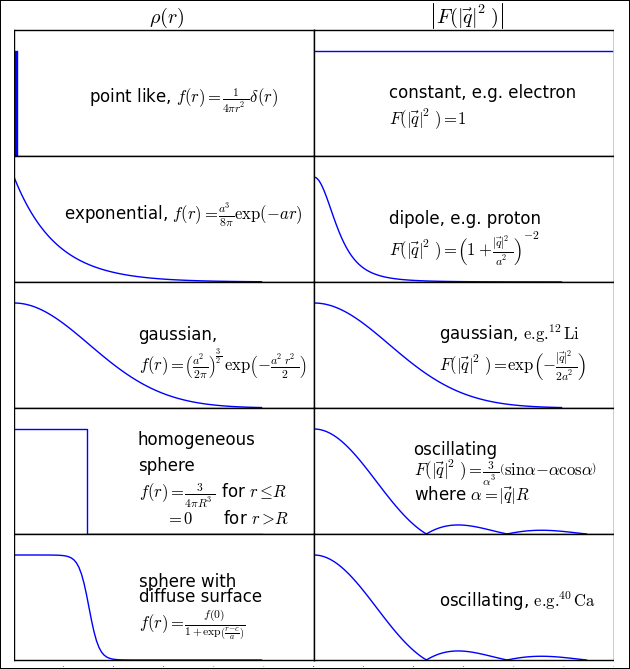
\includegraphics[scale=0.5]{distro.png}
\end{figure}
Key points:
\begin{itemize}
    \item Scattering off an extended charge distribution intoeuces a form factor $F(q)$. $F(q)$ is the Fourier transform of the charge distribution. 
    \item Measure the ration between $d\sigma /d\Omega$ in experiment and Mott allows to determine the shape of $F(q)$.
\end{itemize}

\section{Scattering Off Nucleons}
\begin{itemize}
    \item Require a resolution of $1\,fm = 10^{-15}m$ to perceive nucleons
    \item Requires $q = \frac{\hbar c}{\lambda} = 200\,MeV$
    \item $m_p = 938\,MeV$
    \item For such large momenta, the recoil has to be taken into account: $E \neq E'$
        \begin{equation}
            g(E) = \frac{dn}{dE} = \frac{dn}{dE'}\frac{dE'}{dE} \approx \frac{dn}{dE'}\cdot \frac{E'}{E} = g(E')
        \end{equation}
    \item With this modification, now we have recoil
        \begin{equation}
            \left(\frac{d\sigma}{d\Omega}\right)_{\text{Mott, recoil}} = \left(\frac{d\sigma}{d\Omega}\right)_{\text{Mott, no recoil}} \cdot \frac{E'}{E}
        \end{equation}
    \item The target carries spin, and therefore a magnetic moment. 
        \begin{itemize}
            \item Recall, 
                \begin{equation}
                    \mu = I\cdot A = \frac{q}{2m}L
                \end{equation}
        \end{itemize}
    \item For a spinning charge, 
        \begin{equation}
            \mu = g\frac{e}{M}\cdot S, ~S = \frac{1}{2}
        \end{equation}
\end{itemize}

\chapter{}
Scattering Processes and their cross sections:
\begin{itemize}
    \item pointlike charge (no spin) on pointlike charge (no recoil, no spin) 
        \begin{equation}
            \left(\frac{d\sigma}{d\Omega}\right)_{Ruth} = \frac{e^4z^2Z^2}{4E^2\sin^4(\theta/2)}
        \end{equation}
    \item pointlike charge (spin) on pointlike charge (no recoil, no spin) 
        \begin{equation}
            \left(\frac{d\sigma}{d\Omega}\right)_{\text{Mott, no recoil}} = \left(\frac{d\sigma}{d\Omega}\right)_R \cos^2(\theta/2)
        \end{equation}
    \item pointlike charge (spin) on extended charge (no recoil, no spin) 
        \begin{equation}
            \left(\frac{d\sigma}{d\Omega}\right)_\rho = \left(\frac{d\sigma}{d\Omega}\right)_{\text{Mott, no recoil}} |F(q^2)|^2
        \end{equation}
    \item pointlike charge (spin) on pointlike charge (recoil, no spin) 
        \begin{equation}
            \left(\frac{d\sigma}{d\Omega}\right)_{Mott} = \left(\frac{d\sigma}{d\Omega}\right)_{\text{Mott, no recoil}} \frac{E'}{E}
        \end{equation}
    \item pointlike charge (spin) on pointlike charge (recoil, spin) 
        \begin{equation}
            \left(\frac{d\sigma}{d\Omega}\right) = \left(\frac{d\sigma}{d\Omega}\right)_{Mott} \cdot \left(1 + 2\tau\tan^2(\theta/2)\right)
        \end{equation}
    \item pointlike charge (spin) on extended charge (recoil, spin) 
        \begin{equation}
            \left(\frac{d\sigma}{d\Omega}\right)_{Rosenbluth} = \left(\frac{d\sigma}{d\Omega}\right)_{Mott}\left[\frac{G^2_E(q^2) + \tau G^2_M(q^2)}{1+\tau} + 2\tau G^2_M(q^2)\tan^2(\theta/2)\right]
        \end{equation}
    \item The electric form factor is the Fourier transform of the electric charge distribution. 
        \begin{equation}
            G_E(q^2) = \int e^{iq\cdot y}f(y)\,d^3y
        \end{equation}
    \item The magnetic form factor is the Fourier transform of the magnetic moment distribution. 
        \begin{equation}
            G_M(q^2) = \int e^{iq\cdot y}\mu_z(y)\,d^3y
        \end{equation}
    \item Expectation (for $Q^2 \to 0$) for proton and neutron:
        \begin{align}
            G_E^p &= 1 & G_E^N &= 0 \\
            G_M^p &= 1 & G_M^N &= 0 
        \end{align}
    \item Measurement for proton and neutron:
        \begin{align}
            G_E^p &= 1 & G_E^N &= 0 \\
            G_M^p &= 2.79 & G_M^N &=-1.31
        \end{align}
    \item $G_M^N$ most surprising as neutron should be neutral and not interact magnetically - suggests neutron composed of non-neutral particles
    \item Mind-blowing stuff
        \begin{equation}
            y = mx + c
        \end{equation}
    \item Dipole form factor 
        \begin{align}
            G_E^p, G_M^p, G_M^N &= \frac{1}{1 + \frac{q^2}{a^2}} \\
            G_E^N &= 0
        \end{align}
\end{itemize}

\chapter{}

\chapter{}
\section{Repetition Inelastic Scattering}
\begin{itemize}
    \item 
        \begin{align}
            w_p &= P_\mu + p_\mu + p'_\mu \\
            w^2 &= (P+q)^2 = P^2 + 2P\cdot q - Q^2 \\
                &= M^2 + 2Mv - Q^2 \\
            v &= \frac{P\cdot q}{M}
        \end{align}
    \item Further increasing the energy leads to inelastic scattering.
        Now the target can become excited and additional particles are produced.
        We need two parameters to describe the cross section.
    \item Deep inelastic scattering 
        \begin{align}
            \frac{d^\sigma}{d\Omega\,dE'} = \left(\frac{d\sigma}{d\Omega}\right)_{\text{Mott, no recoil}} \left[W_2(Q^2,v) + 2W_1(Q^2,v)\tan^2\frac{\theta}{2}\right]
        \end{align}
        $W_i$ are known as structure functions - they are the "form factors" of inelastic scattering.
    \item Choose dimensionless structure functions. 
        Define, 
        \begin{align}
            x &= \frac{Q^2}{2Mv} \\
            2Mv &- Q^2 \geq 0 \\
            0 &< x \leq 1
        \end{align}
        $x$ is the Bjorken scale variable. 
    \item $F_1$ is the magnetic ff, and $F_2$ is electric
        \begin{align}
            F_1(x,Q^2) &= MW_1(Q^2,v) \\
            F_2(x,Q^2) &= vW_2(Q^2,v)
        \end{align}
    \item Expressed in dimensionless structure functions, the cross section reads
        \begin{align}
            \frac{d^2\sigma}{dxdQ^2} &= \frac{4\pi\alpha^2}{Q^4}\left[\left(1-y-\frac{M^2x^2y^2}{Q^2}\right)\frac{F_2(x,Q^2)}{x} + \frac{y^2}{2}\frac{2xF_1(x,Q^2)}{x}\right] \\
            y &= \frac{P\cdot q}{p\cdot q}
        \end{align}
    \item In elastic scattering, both form factors of the proton are proportional to a dipole
        \begin{align}
            \sigma &\propto |G_{dipol}|^2 \propto \frac{1}{Q^3} \\
            G_{dipol} &= \frac{1}{\left(1-\frac{|q|^2}{a^2}\right)^2}
        \end{align}
    \item What do we observe for large momenta?
        The structure functions are apprxoimately flat in $Q^2$. 
        This hints at a point-like substructure of the proton.
    \item What about the x dependence?
        \begin{itemize}
            \item Use $R$ as the radius of the proton
            \item $Q^2R^2 << 1$ is the regime of elastic scattering, $x=1$.
            \item $Q^2R^2 \approx 1$, we start seeing structure and can excite proton to higher energy states.
            \item $Q^2R^2 >> 1$, can look deep into the structure of the proton.
        \end{itemize}
        \begin{figure}[H]
            \centering
            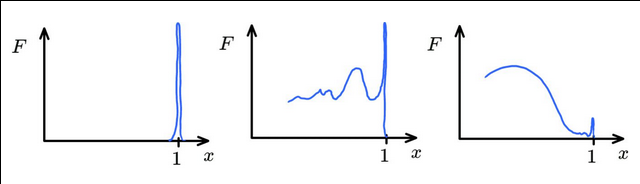
\includegraphics[scale=0.5]{forms.png}
        \end{figure}
    \item Key points
        \begin{itemize}
            \item In a Deep Inelastic Scattering experiment, one collides large energy electrons with a proton. 
            \item There are 3 scattering regimes
            \item Low energy $Q^2R^2 << 1$ is eleastic scattering
            \item Moderate energy $Q^2R^2 \approx 1$ yields resonances
            \item High energy $Q^2R^2 >> 1$ yields point-like substructure
        \end{itemize}
    \item Parton model - there were hints of point-like substructure which were just called partons at first
    \item Assume that each parton carries a fraction of the Proton momentum, $P$.
        For massless ($0 \leq \eta \leq 1$) partons with momentum $k = \eta P$.
        \begin{align}
            0 = k^2 &= (\eta P + p-p')^2  = (\eta P + q)^2 \\
                    &= \eta^2M^2 + 2\eta P\cdot q - Q^2
        \end{align}
        Assume $Q^2 >> M^2$:
        \begin{align}
            \eta &= \frac{Q^2}{2P\cdot q} = x
        \end{align}
    \item This gives a physical interpretation of what $x$ is - it is the fraction of the proton momentum carried by the individual parton that is struck in the scattering. 
    \item Looking at the right-most figure above, the highest peak is at $x \approx 1/3$, suggesting that each parton has mass $m_p/3$, and therefore there must be three of them - assuming no one parton is any more special than the others. 
\end{itemize}

\chapter{}
\begin{itemize}
    \item What is the parton spin?
        For spin $\frac{1}{2}$, 
        \begin{equation}
            F_2(x,Q^2) = 2xF_1(x,Q^2)
        \end{equation}
        This is the Callan-Gross relation.
    \item The differential cross-section can be rewritten as
        \begin{align}
            \frac{d\sigma}{dQ^2dx} &= \sum_{\text{constituents}} f_c(x)\frac{d\sigma}{d\Omega}(e^-,c;p,x,P,p')
        \end{align}
    \item $f_c(x)$ is the parton distribution function.
        This is the number of partons of type $c$ with momentum fraction in an infinitesimal interval around $x$.
        \begin{equation}
            dn_c(x) = f_c(x)\,dx
        \end{equation}
    \item The structure functions can now be expressed as
        \begin{align}
            F_2(x,Q^2) &= 2xF_1(x,Q^2) \\
                       &= x\sum_{\text{constituents}} Q^2_cf_c(x)
        \end{align}
    \item Quarks 
        \begin{table}[H]
            \centering
            \begin{tabular}{l|c|c}
                Name    & Symbol & Charge \\
                \hline
                up      & u      & $+\frac23$ \\
                down    & d      & $-\frac13$ \\
                \hline
                strange & s      & $-\frac13$ \\
                charm   & c      & $+\frac23$ \\
                \hline
                bottom  & b      & $-\frac13$ \\
                top     & t      & $+\frac23$
            \end{tabular}
        \end{table}
    \item Gluons are the force carriers of the strong force. 
        In contrast to photons, they self-interact.
    \item Can draw similar field lines to that of electromagnetism dipoles, but field lines increase in density as you pull them apart, until you've provided enough energy by pulling them apart to generate new particles, which form new bound states with the old quarks, i.e. pions
    \item Nuclear decay arises due to short range of strong force but infinite range of electromagnetism - eventually over a large enough nucleus, the strength of the summed electromagnetic repulsion overcomes the strong force coupling.
    \item Partons can be produced for a short amount of time through Heisenberg uncertainty, $\delta E\delta t \geq \frac{\hbar}{2}$. 
        These are known as sea quarks.
        \begin{itemize}
            \item Quark-antiquark pairs can form as part of a nucleon for a short amount of time as they do not change the overall charge
            \item The higher the mass of the quarks, the less likely they are to form $\implies$ higher mass requires more energy, so smaller lifetime
        \end{itemize}
    \item We cann predict parton distribution functions from first principles, but some can be derived.
        \begin{itemize}
            \item Using all constituents
                \begin{align}
                    \int_0^1 \sum_c xf_x(x)\,dx = 1
                \end{align}
            \item Using charged constituents
                \begin{equation}
                    \int_0^1 \sum_{\text{quarks} = q} Q_qf_q(x)\,dx = 1
                \end{equation}
                That $1$ is the proton charge.
        \end{itemize}
        \begin{align}
            f_q(x) = f_q^v(x) + f_q^s
        \end{align}
        Assume no gluons and $f_q^s(x) = 0$.
        \begin{figure}[H]
            \centering
            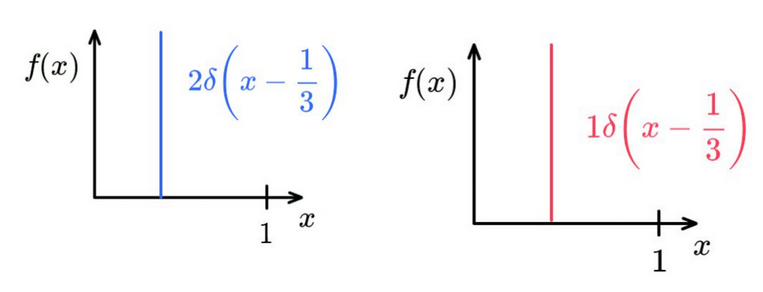
\includegraphics[scale=0.5]{pdf1.png}
        \end{figure}
    \item What if the 2 up-quarks share $\frac12$ of the momentum and the down quark carries the other $\frac12$?
        \begin{figure}[H]
            \centering
            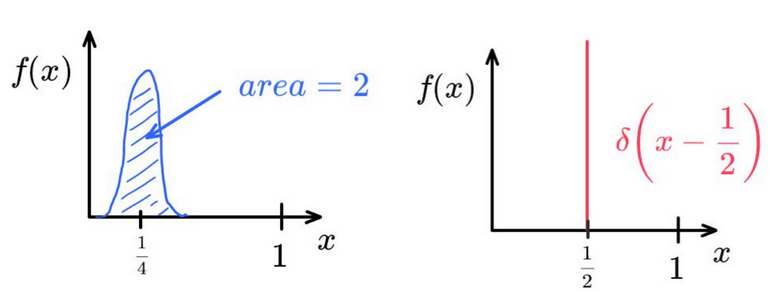
\includegraphics[scale=0.5]{pdf2.png}
        \end{figure}
    \item Educated guess
        \begin{align}
            f(x) &= x^a(1-x)^b, ~a,b > 0 \\
            \lim_{x\to0} &f(x) = 0 \\
            \lim_{x\to1} &f(x) = 0 
        \end{align}
        Tells us that they cannot be at rest and cannot carry all the momentum.
\end{itemize}

\chapter{}
\begin{itemize}
    \item The parton model stipulates that the proton is made up from constituent particles called partons (quarks)
    \item Callan-Gross relation implies partons carry spin-$\frac12$
    \item The constituents carry momentum fractions described the PDFs
    \item There are two types of quark in the nucleon
        \begin{itemize}
            \item Valence quarks that determine the quantum numbers
            \item Ion quarks that appear in $q-\bar{q}$ pairs
        \end{itemize}
\end{itemize}

\section{Quark Structure of the Nucleus}
\begin{itemize}
    \item Consider $e^-p$ scattering
        \begin{equation}
            F_2(x) = x\sum_f Q_f^2(q_f(x) + \bar{q}_f(x)) 
        \end{equation}
        \begin{align}
            \begin{split}
                F_2(x) &= x\Bigg[\frac{1}{9}\left(d_v^p(x) + d_s^p(x) + \bar{d}_s^p(x)\right) \\ &+ \frac{4}{9}\left(u_v^p(x) + u_s^p(x) + \bar{u}_s^p(x)\right) \\ &+ \frac{1}{9}\left(s_s^p(x) + \bar{s}_s^p(x)\right) + \cdots \Bigg] 
        \end{split}
        \end{align}
    \item Can use relations
        \begin{align}
            u_v^p &= d_v^n & d_v^p &= u_v^n & s_s^p &= s_s^n 
        \end{align}
    \item Now $e^-n$ scattering - similar with more down quarks than up quarks, use the above relations to give it the same variables
        \begin{align}
            \begin{split}
                F_2^{en}(x) &= x\bigg[\frac19\left(d_v^n + d_s^n + \bar{d}_s^n\right) \\ &+ \frac49\left(u_v^n + u_s^n + \bar{u}_s^n\right) \\ &+ \frac19\left(s_s^n + \bar{s}_s^n\right)\bigg]
            \end{split}\\
            \begin{split}
                F_2^{en}(x) &= x\bigg[\frac19\left(u_v^p + u_s^p + \bar{u}_s^p\right) \\ &+ \frac49\left(d_v^n + d_s^p + \bar{d}_s^p\right) \\ &+ \frac19\left(s_s^p + \bar{s}_s^p\right)\bigg]
            \end{split}
        \end{align}
    \item Can take the average of these two 
        \begin{align}
            \begin{split}
                F_2^{eN} = \frac{F_2^{ep} + F_2^{en}}{2} &= x\bigg[\frac{5}{18}\left(d_v^p + d_s^p + \bar{d}_s^p\right) \\ &+ \frac{5}{18}\left(u_v^p + u_s^p + \bar{u}_s^p\right) \\ &+ \frac19\left(s_s^p + \bar{s}_s^p\right)\bigg]
            \end{split}
        \end{align}
    \item Now we turn our eyes to the mystical creature known as the neutrino - cousin to the mighty unicorn
        \begin{equation}
            F_2^{\nu N} = x\sum_f (q_f(x) + \bar{q}_f(x))
        \end{equation}
    \item We neglect the strange quark
        \begin{equation}
            \frac{F_2^{eN}}{F_2^{\nu N}} = \frac{5}{18}
        \end{equation}
    \item Now look at the momentum distribution - $q_f(x)$ (or $f_(x)$) is the probability of finding a parton with a momentum fraction $x\cdot\unl{P}$, where $\unl{P}$ is the momentum of the proton. 
        We can estimate the momentum carried by the quarks $f$ and anti-quarks $\bar{f}$.
        \begin{align}
            p_f &= \int_0^1 (q_f(x) + \bar{q}_f(x))x\unl{P}\,dx
        \end{align}
    \item The fraction of the total momentum carried by quarks is then
        \begin{align}
            \frac{\sum_f p_f}{\unl{P}} &= \sum_f \int_0^1 x(q_f(x) + \bar{q}_f(x))\,dx \\
                                       &= \int_0^1 F_2^{\nu N}(x)\,dx = \frac{18}{5}\int_0^1 F_2^{eN}(x)\,dx
        \end{align}
        If there were only quarks, this would be $= 1$. 
        The fact that it is $\approx 0.5$ is indirect evidence of gluons. 
    \item Gluons will decay into a quark and antiquark which can then recombine into a gluon again so depending on when you take your measurement, the part of the momentum not occupied by normal quarks could either be gluons or sea quarks.
\end{itemize}

\section{Colour}
\begin{itemize}
    \item Up, down, and strange quarks have been introduced to understand the properties of baryons (3 quarks).
        \begin{itemize}
            \item 2 ups, 1 down - proton
            \item 1 up, 2 downs - neutron
            \item 2 ups, 1 strange - $\Sigma^+$ (+1 nuclear charge)
            \item 3 ups - $\Delta^{++}$ (+2 nuclear charge)
        \end{itemize}
    \item How to explain the $\Delta^{++}$ with all three spins aligned? What about Pauli?
    \item The strong charge is called colour. 
            \item For the $\Delta^{++}$, the three up quarks have the same spins, but one is red-, one is blue-, one is green- colour-charged
    \item Gluons carry colour-anticolour combinations, i.e. red-antigreen
        \begin{figure}[H]
            \centering
            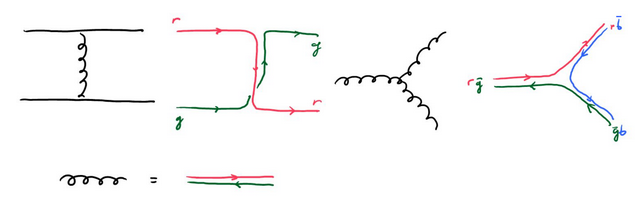
\includegraphics[scale=0.5]{colour.png}
        \end{figure}
    \item The experimental consequence is that only globally colour-neutral particles can be observed.
\end{itemize}

\chapter{}
\begin{itemize}
    \item We can get information about the PDFs using DIS with different targets and projectiles
    \item The total function of momentum carried by quarks is $\approx 0.5$. 
        The other half is carried by gluons.
    \item The $\Delta^{++}$ resonance only agrees with the Pauli Principle, if we introduce \textbf{colour.}
    \item Both quarks and gluons carry colour. 
    \item Gluons mediate the strong force. 
    \item Only colour-neutral objects above $\approx$ 1 fm.
\end{itemize}
\begin{figure}[H]
    \centering
    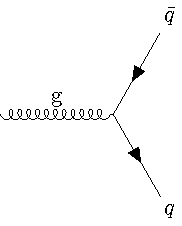
\includegraphics{gluon1.pdf}
    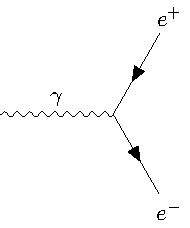
\includegraphics{gluon2.pdf}
\end{figure}

\section{Scaling Violation}
There is a mild $Q^2$-dependence in the PDFs, because the "resolution" of the photon in deep inelastic scattering is increasing with $Q^2$ revealing more sea quarks and gluons than at low $Q^2$.
\begin{figure}[H]
    \centering
    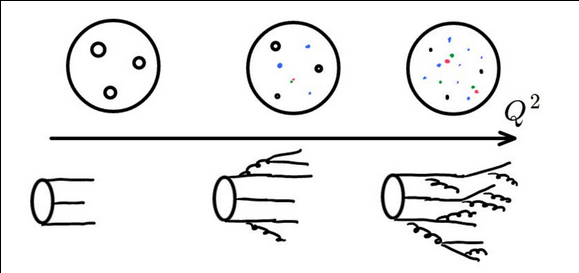
\includegraphics[scale=0.5]{scale.png}
\end{figure}

\section{Feynman Diagrams}
Feynman diagrams are a way of illustrating interactions in particle physics.
\begin{itemize}
    \item Fermions are represented by plain lines. Arrows in direction of time represent fermions. Arrows against the direction of time represent anti-fermions.
        \begin{figure}[H]
            \centering
            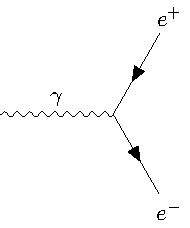
\includegraphics{gluon2.pdf}
        \end{figure}
    \item Bosons
        \begin{itemize}
            \item Electroweak bosons are wiggly lines
                \begin{figure}[H]
                    \centering
                    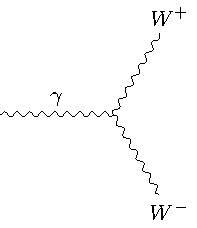
\includegraphics{w1.pdf}
                \end{figure}
            \item Strong (gluons) is curly
                \begin{figure}[H]
                    \centering
                    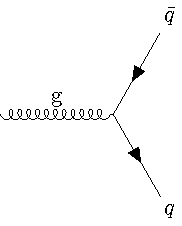
\includegraphics{gluon1.pdf}
                \end{figure}
            \item Higgs is dashed
                \begin{figure}[H]
                    \centering
                    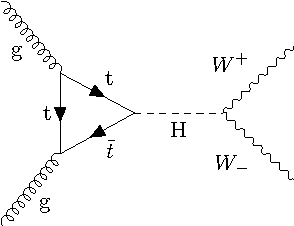
\includegraphics{higgs1.pdf}
                \end{figure}
        \end{itemize}
    \item Vertices - interaction points. Each vertex conserves:
        \begin{itemize}
            \item Electric charge
            \item Lepton number
        \end{itemize}
    \item Photons couple to all electrically charged particles.
        Each vertex carries $Q\sqrt{\alpha}$ with $\alpha = \frac{e^2}{4\pi} = \frac{1}{137}$.
    \item W-Boson - All W-interactions have a different strength depending on the flavours involved.
    \item The Z-Boson couples to all weak charges. 
    \item The gluon couples to all coloured particles with an interaction strength of $\sqrt{\alpha_s}$.
    \item Internal Particles: 
        \begin{figure}[H]
            \centering
            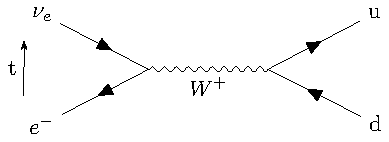
\includegraphics{int1.pdf}
        \end{figure}
        Internal lines bring a factor
        \begin{equation*}
            \frac{1}{p^2-m^2+im\Gamma}
        \end{equation*}
    \item Standard model vertices - 4-vertices and Higgs interactions.
\end{itemize}

\chapter{}

\section{How to draw a Feynman diagram}
\begin{enumerate}
    \item Start with fermion lines
    \item Dress it with the right bosons
\end{enumerate}

Key points:
\begin{itemize}
    \item All vertices conserve:
        \begin{itemize}
            \item electric charge
            \item Baryon number
            \item Lepton number
        \end{itemize}
\end{itemize}

\section{Quarkonia}
Just like $e^-p+$ and $e^+e^-$ can form bound states under electromagnetism, so can $q\bar{q}$ pairs under the strong force.
Explore the spectrum of ($c\bar{c}$) and ($b\bar{b}$) states to learn about the $q-\bar{q}$ potential. 
Produced by:
\begin{figure}[H]
    \centering
    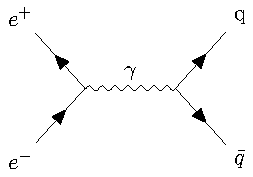
\includegraphics{charm}
\end{figure}
Set energy of $e^+e^-$ right $\to$ produce resonances.
Lowest lying resonance (lightest) $J/\psi = (\bar{c}c),\, m_{J/\psi} = 3.097\,\text{GeV}$ (3$\times$ proton mass) - $J/\psi = 1^-$.
Heavier states decay into lighter states through radiating off a photon in analogy to $e^+e^-,\,e^-p^+$.

This "fine-structure" splitting between the two 1S states in $e^+e^-$ originates from spin-spin interactions.
\begin{align}
    V_{ss}(e^+e^-) &= \frac{8\pi}{3}\alpha\frac{\vec{S}_1\cdot\vec{S}_2}{m_e^2}\delta(\vec{x}) \\
    V_{ss}(q\bar{q}) &= \frac{32\pi}{9}\alpha_s\frac{\vec{S}_q\cdot\vec{S}_{\bar{q}}}{m_qm_{\bar{q}}}\delta(\vec{x})
\end{align}
To calculate the energy or mass shift between the two 1S states, we need the value of $\langle \vec{S}_1\cdot\vec{S}_2\rangle$:
\begin{align}
    S(S+1) &= \langle (S_1 + S_2)^2\rangle \\
           &= \langle S_1^2\rangle + 2\langle S_1\cdot S_2\rangle + \langle S_2^2\rangle \\
           &= \frac12 (\frac12 + 1) + 2\langle S_1\cdot S_2\rangle + \frac12 (\frac12 + 1) \\
           &= \frac32 + 2\langle S_1\cdot S_2\rangle \\
    \implies \langle S_1\cdot S_2\rangle &= \frac{2S(S+1) - 3}{4} = \begin{cases} -\frac34 & S = 0 \\ \frac14 & S = 1 \end{cases} \\
    E_{ss} &= \langle\psi|V_{ss}|\psi\rangle = \frac{8\pi\alpha_s}{gm_qm_{\bar{q}}}\langle\psi|\delta(\vec{x})|\psi\rangle \begin{cases} -3 \\ 1 \end{cases} \\ 
           &= \frac{8\pi}{gm_q^2}|\psi(0)|^2\begin{cases} -3 \\ 1 \end{cases}
\end{align}
The mass split, 
\begin{align}
    \Delta E_{ss} &= E_{ss}(S=1) - E_{ss}(S=0) \\
                  &= \frac{32\pi}{g}\frac{\alpha_s}{m_q^2}|\psi(0)|^2
\end{align}

\section{Quark-Antiquark Potential}
For small distances, 
\begin{equation}
    V(r) \propto \frac{1}{r}
\end{equation}
For large distances, $V(r)$ has to grow. 
\begin{equation}
    V(r) = \underbrace{-\frac43\frac{\alpha_s(r)}{r}}_{\text{short-range}} + \underbrace{kr}_{\text{long-range}}
\end{equation}


\chapter{}
\begin{itemize}
    \item Four ways for Quarkonia to decay:
        \begin{itemize}
            \item  EM decays 
            \item virtual/real photon emission and gluon emission
            \item Decays through quarkonia production
            \item Weak decays (change of quark)
        \end{itemize}
    \item Parity is the spatial inversion at the origin
        \begin{align}
            \psi(x,t) \to \psi'(x,t) = \hat{P}\psi(x,t) = \psi(-x,t) \\
        \end{align}
    \item Parity is conserved in QED (photons) and QCD (gluons), not in weak interactions (W,Z)
    \item All (anti-)fermions in the Standard Model have $P(\psi) = 1,~ P(\bar{\psi}) = -1$
    \item Vector bosons have $P(\gamma) = P(g) = P(W^{\pm}) = P(Z) = -1$
    \item $P(\vec{E}) = -1,~ P(\vec{B}) = 1$
\end{itemize}

\section{EM Decays}
For a state $n^{2S+1}L_J$, parity is given by
\begin{equation}
    P(n^{2S+1}L_J) = \underbrace{P(q)P(\bar{q})}_{-1}(-1)^L = (-1)^{L+1}
\end{equation}

Key points:
\begin{itemize}
    \item Charm-anticharm bound states are charmonium
    \item Bottom-antibottom bound states are bottomium
    \item The spectrum of these states teaches us about the quarkonium potential
    \item At small distances, $V_{q\bar{q}} \propto \frac{1}{r}$
    \item At large distances, $V_{q\bar{q}} \propto r$
    \item Large $L=0$ splittings are a result of spin-spin interactions
    \item There are four decay channels:
        \begin{itemize}
            \item De-excitation (photon decay)
            \item Virtual gluon/photon decay (several)
            \item Hadronic (split into more quarkonia of lower mass)
            \item Weak interaction (change of quark)
        \end{itemize}
\end{itemize}

\chapter{}
\section{Light Quark Mesons (u,d,s)}
These are more complicated, because the motion of the light quarks in the bound state is relativistic. 
Additional tool: symmetry $u \leftrightarrow d \leftrightarrow s$.

\subsection{Properties of Light Mesons}
Consider $L=0$ states (1S).
\begin{itemize}
    \item Parity
        \begin{equation}
            P = \underbrace{P(\bar{q})P(q)}_{-1}(-1)^L = -1
        \end{equation}
    \item $L + S = J$, $J^P = O^-$ - pseudoscalar mesons
    \item $J^P = 1^-$ vector mesons
    \item We have 3 light quarks (u,d,s) and 3 light anti-quarks ($3\times3=9$)
    \item For massless quarks, there is a symmetry: $u \leftrightarrow d \implies$ Isospin
\end{itemize}

\subsection{Isospin}
The Isospin operator is the same as the spin operator, but it acts on flavour: $I_a = \frac{\sigma_a}{2}$.
\begin{align}
    I_1 &= \frac12 \begin{pmatrix} 0 & 1 \\ 1 & 0 \end{pmatrix} & I_2 &= \frac12\begin{pmatrix} 0 & -i \\ i & 0 \end{pmatrix} & I_3 &= \frac12 \begin{pmatrix} 1 & 0 \\ 0 & -1\end{pmatrix} 
\end{align}
\begin{align}
    I^2 &= I_1^2 + I_2^2 + I_3^2,~ EV = I(I+1) \\
    \begin{pmatrix} u \\ d\end{pmatrix} &\implies I_3 = \begin{cases} +\frac12 \\ -\frac12\end{cases},~ I = \frac12 \\
    \begin{pmatrix} -\bar{d} \\ \bar{u}\end{pmatrix} &\implies I_3 = \begin{cases} +\frac12 \\ -\frac12 \end{cases},~ I = \frac12
\end{align}
For spin: 
\begin{equation}
    \frac12 \otimes \frac 12 = 0 \oplus 1
\end{equation}
Now: 
\begin{equation}
    2\otimes \bar{2} = 1 \oplus 3
\end{equation}
\begin{figure}[H]
    \centering
    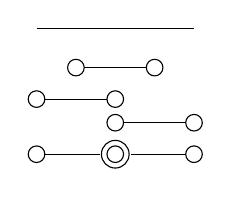
\begin{tikzpicture}
        \draw (-1,4) -- (1,4);
        \draw (-1/2,3.5) circle (3pt);
        \draw (1/2,3.5) circle (3pt);
        \draw (-0.4,3.5) -- (0.4,3.5);
        \draw (-1,3.1) circle (3pt);
        \draw (0,3.1) circle (3pt);
        \draw (-0.9,3.1) -- (-0.1,3.1);
        \draw (0,2.8) circle (3pt);
        \draw (1,2.8) circle (3pt);
        \draw (0.1,2.8) -- (0.9,2.8);
        \draw (-1,2.4) circle (3pt);
        \draw (-0.9,2.4) -- (-0.2,2.4);
        \draw (0,2.4) circle (3pt);
        \draw (0,2.4) circle (5pt);
        \draw (0.2,2.4) -- (0.9,2.4);
        \draw (1,2.4) circle (3pt);
    \end{tikzpicture}
\end{figure}

\section{Meson Multiplets}
We can decompose the tensor-product of a triplet and an anti-triplet under SU(3).
\begin{equation}
    3 \otimes 3 = 8 \oplus 1
\end{equation}
Graphical representation: what is going on?

\section{Meson Masses}
Vector mesons are heavier due to the spin-spin interactions.
\begin{equation}
    E_{ss} = \frac{8}{9}\frac{\pi \alpha_s}{m_qm_{\bar{q}}}|\psi(0)|^2 \begin{cases} -3 & J = 0 \\ 1 & J = 1\end{cases}
\end{equation}
Assume $m_u = m_d$ and $|\psi(0)|^2$ is roughtly the same $\implies$
\begin{align}
    m_{u,d} &\approx 310\,MeV,~ m_s \approx 483\,MeV \\
    m_{\text{constituent}} &= m_{\text{intrinsic}} + m_{\text{dynamic}}
\end{align}
Lighter quarks are mainly dynamic mass, heavier quarks mainly intrinsic mass.

\chapter{}

\chapter{}
\section{Lepton Pair Production}
\begin{itemize}
    \item \textit{put some Feynman diagrams in here}
    \item $e^-$ are stable
    \item $\mu^-$ are unstable - rather long-lived on these scales, $t_\mu \approx 2\mu s$
    \item $\tau^-$ are unstable - short-lived, $t_\tau \approx 3\times10^{-13}s$
\end{itemize}

\section{Hadron Production}
\begin{itemize}
    \item \textit{some Feynman diagrams here}
    \item Leptons have $Q=-1$, Quarks have $Q=-\frac13,\frac23$
    \item Quarks carry colour quantum numbers: red, green, blue
        \begin{align}
            \sigma(e^+e^-\to\text{ hadrons}) &= \sum_f \sigma(e^+e^-\to q_f\bar{q}_f)\Theta(\sqrt{s}-2m_f) \\
            \sigma(e^+e^-\to q_f\bar{q}_f) &= N_cQ_f^2\sigma(e^+e^-\to\mu^+\mu^-)
        \end{align}
    \item $N_c$ is the number of colours (3)
    \item Can take the ratio
        \begin{align}
            R &= \frac{\sigma(e^+e^-\to \text{ hadrons})}{\sigma(e^+e^-\to\mu^+\mu^-)} \\
              &= 3\sum_{2m_f\leq\sqrt{s}} Q_f^2
        \end{align}
        \begin{align}
            \sqrt{s} &> 2m_s & R &= 3\left(\frac49+\frac19+\frac19\right) = 2 \\
            \sqrt{s} &> 2m_c & R &= 3\left(\frac49+\frac19+\frac19+\frac49\right) = \frac{10}{3} \\
            \sqrt{s} &> 2m_b & R &= 3\left(\frac49+\frac19+\frac19+\frac49+\frac19\right) = \frac{11}{3}
        \end{align}
\end{itemize}
\begin{figure}[H]
    \centering
    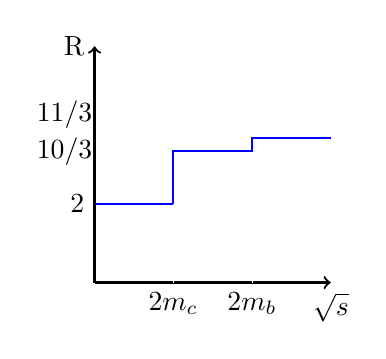
\begin{tikzpicture}
        \draw[thick,->] (0,0) -- (0,3) node[anchor=east] {R};
        \draw[thick,->] (0,0) -- (3,0) node[anchor=north] {$\sqrt{s}$};
        \draw[thick,blue] (0,1) node[anchor=east,black] {2} -- (1,1) -- (1,5/3) -- (2,5/3) -- (2,11/6) -- (3,11/6);
        \draw[white] (1,0) node[anchor=north,black] {$2m_c$} -- (1,1);
        \draw[white] (2,0) node[anchor=north,black] {$2m_b$} -- (2,1);
        \draw[white] (0.2,5/3) node[anchor=east,black,xshift=-3pt] {10/3} -- (0.2,11/6) node[anchor=south east,black,xshift=-3pt] {11/3};
    \end{tikzpicture}
\end{figure}
The differential cross section
\begin{align}
    \frac{d\sigma(e^+e^-\to\mu^+\mu^-)}{d\Omega} &= \frac{\alpha^2}{4s}(1+\cos^2\theta) \\
    \sigma &= \frac{4\pi}{3}\alpha^2\frac{1}{s}
\end{align}
Neglect the Z-Boson
\begin{align}
    \mu &\propto \frac{1}{q^2-M_\mu^2} + \frac{1}{q^2-M_Z^2} \\
        &= \frac{1}{s} - \frac{1}{M_Z^2} \\
    \sigma &\propto S\left(\frac{1}{s} - \frac{1}{M_Z^2}\right)^2 = \frac{1}{S} - \frac{2}{M_Z^2} + \frac{s}{M_Z^4} = \frac{1}{S}
\end{align}

\section{Resonances}
\textit{Put Feynman diagram in here}
\begin{itemize}
    \item Virtual photons can only produce resonances of $q\bar{q}$ pairs with $Q_R = 0$ and $J_R = 1$.
\end{itemize}

\chapter{}
\section{Key Point}
\begin{itemize}
    \item $e^+e^-$ collisions are clean (initial state has a well-defined center-of-mass energy, no structure functions)
    \item Hadron production in $e^+e^-$ collisions occur through the production of $q-\bar{q}$ pairs, for $\sqrt{s} \geq 2m_q$ ($\sqrt{s}$ the center-of-mass energy), compatible with $\gamma^*$, $J^p = 1^-$
    \item The R-ratio,
        \begin{equation}
            \frac{\sigma(e^+e^-\to\text{hadrons})}{\sigma(e^+e^-\to\mu^+\mu^-)},
        \end{equation}
        shows the quark thresholds and yields information on the number of colours, $N_c = 3$, and the quark charges
    \item At $91.2\,GeV$, the Z-boson is produced on-shell
    \item The heigh of the resonance peak is related to its width
        \begin{align}
            \sigma &= \frac{1}{(p^2+M_Z^2) + \Gamma^2M_Z^2} \propto \left(\lim_{p^2\approx M_Z^2}\right) \frac{1}{\Gamma^2} \\
            \Gamma_{tot} &= \Gamma(Z\to e^+e^-) + \Gamma(Z\to\mu^+\mu^-) + \Gamma(Z\to\tau^+\tau^-) + \Gamma(Z\to q\bar{q}) + \Gamma(Z\to\nu\bar{\nu})
        \end{align}
\end{itemize}

\section{Weak Interaction}
\begin{center}
    \begin{tabular}{c|c|c}
        Name & Interaction & Mass \\
        \hline
        Photon, $\gamma$ & E/M & 0 \\
        Gluons, g & strong & 0 \\
        $W^{\pm},\,Z$ & weak & $80.4\,GeV,\; 91.2\,GeV$
    \end{tabular}
\end{center}
Why weak?
Interactions are suppressed by the heavy mediator masses.\\
Which particles take part in the weak interaction?

\subsection{Charged Leptons}
\begin{center}
    \begin{tabular}{c|c|c}
        Name & Mass & Charge \\
        \hline
        $e^-$ & $0.511\,MeV$ & $-1$ \\
        $\mu^-$ & $105.65\,MeV$ & $-1$ \\
        $\tau^-$ & $1776.8\,MeV$ & $-1$
    \end{tabular}
\end{center}
Charged leptons share all quantum numbers apart from mass.
If leptons were composite, you would expect $\mu \to e\gamma$, but this has never been observed.
They decay through other channels:
\begin{align}
    \mu^- &\to e^-\bar{\nu}_e\nu_\mu \\
    \tau^- &\to e^-\bar{\nu}_e\nu_\tau \\
           &\to \mu^-\bar{\nu}_\mu\nu_\tau \\
           &\to \pi^-\nu_\tau
\end{align}
\textit{draw some Feynman diagrams here for tau to pion and mu to electron.}

\subsection{Neutrinos}
\begin{itemize}
    \item Almost massless, $m_\nu < 2\,eV$
    \item electrically neutral
    \item colour-less
    \item Introduced because of $\beta$-decay
        \begin{equation}
            n \to p + e^- + \bar{\nu}_e
        \end{equation}
    \item Anti-neutrinos are produced by reactions
        \begin{align}
            \bar{\nu}_e + p &\to n + e^+ \\
            \nu_e + n &\to p + e^-
        \end{align}
        The first has been observed, while the second is not observed. 
        Therefore, $\bar{\nu}_e \neq \nu_e$.
    \item Each charged lepton comes with a neutrino partner
        \begin{align}
            \begin{pmatrix} e^- \\ \nu_e\end{pmatrix},~  \begin{pmatrix} \mu^- \\ \nu_\mu\end{pmatrix},~ \begin{pmatrix} \tau^- \\ \nu_\tau\end{pmatrix}
        \end{align}
    \item Lepton number is conserved
        \begin{align}
            L_l &= N(l) - N(\bar{l}) +  N(\nu_l) - N(\bar{\nu}_l) \\
            L &= L_e + L_\mu + L_\tau
        \end{align}
\end{itemize}

\chapter{}
\section{Coupling Strength of the Weak Interaction}
\begin{align}
    \frac{g^2}{q^2-M_W^2} &= g^2\left(-\frac{1}{M_W^2} - \frac{g^2}{M_W^2} + \cdots\right)
\end{align}
\begin{itemize}
    \item Contracting the W-propagator
        \begin{equation}
            \frac{G_F}{\sqrt{2}} = \frac{g^2}{M_W^2}
        \end{equation}
    \item $G_F$ is the Ferm constant
\end{itemize}

\section{Quarks and the CKM matrix}
It should also be possible to extract the Fermi constant from semi-leptonic processes.

\section{Key Points}
\begin{itemize}
    \item Weak interaction is mediated by $W^\pm$ and $Z$ bosons
    \item It is responsible for $\beta$ decay, and the decays of heavy quarks and leptons
    \item There are 3 charged leptons and 3 neutrinos
    \item Leptons can be organised in generations, like quarks, with a neutrino associated with each of the charged leptons
    \item Lepton number is conserved for each generation, and therefore total lepton number also
    \item Weak interactions can be charged ($W^\pm$), or neutral ($Z$)
    \item $Z$ interactions never change flavour; charged interactions can change quark flavour, because the mass basis and the weak basis are not the same
    \item Flavour changing transitions are proportional to CKM elements
\end{itemize}

\chapter{}
\section{Parity Violation}
Parity is the symmetry associated with space inversion.
\begin{align}
    \vx &\to -\vx,\text{ vector} \\
    \vp &\to -\vp,\text{ vector} \\
    \vec{L} = \vx\times\vp &\to (-\vx)\times(-\vp)=\vec{L},\text{ axial vector} \\
    E_{kin} = \frac12 m\vx^2 &\to \frac12 m(-\vx)^2 = E,\text{ scalar} \\
    h = \frac{\vec{s}\cdot\vp}{|\vec{s}||\vp|} &\to \frac{\vec{s}\cdot(-\vp)}{|\vec{s}||(-\vp)|} = -h,\text{pseudo-scalar}
\end{align}
For a massless fermion, helicity (spin along direction of momentum) is conserved, either as $h=+1$ for along momentum (right-handed), or $h=-1$ for anti-along the momentum (left-handed).\\
Remember Mott scattering
\begin{align}
    \left(\frac{d\sigma}{d\Omega}\right)_{Mott} &= \left(\frac{d\sigma}{d\Omega}\right)_{Ruth}\cos^2\theta
\end{align}
Helicity changes sign from scattering, so must have mass.\\
What happens to anti-fermions?
\textit{Draw Feynman diagrams in lecture 29 on notes.}
The amplitude of the two diagrams are equivalent, so left-handed fermions and right-handed anti-fermions must be equivalent.
Interactions can be classified like vectors (axial-vectors) depending on left- and right-handed fermions and anti-fermions.
\begin{itemize}
    \item \textbf{Vector interactions} only couple between the same handedness ($f_L$ and $f_L$, or $f_L$ and $\bar{f}_R$, or $\bar{f}_R$ and $\bar{f}_R$, etc)
    \item \textbf{Axial-vector interactions} have couplings between opposite handedness ($f_L$ and $f_R$, or $f_L$ and $\bar{f}_L$, etc)
\end{itemize}
Each interaction can be split up into a vector part ($c_V$) and an axial-vector part ($c_A$).
If $c_V=0,c_A\neq0$ or $c_A=0,c_V\neq0$, parity is conserved.\\
If $c_A=c_V$, the so-called $V+A$ interaction, only $f_R-\bar{f}_L$ couplings exist and $f_L-\bar{f}_R$ couplings are forbidden. \\
If $c_A=-c_V$, the so-called $V-A$, only $f_L-\bar{f}_R$ interact, and $f_R-\bar{f}_L$ is forbidden.\\
$V-A$ and $V+A$ interactions maximally violate parity.
In the standard model:
\begin{center}
    \begin{tabular}{c|c|c}
        Force & Carrier & Coupling \\
        \hline
        EM & $\gamma$ & $c_A=0$ \\
        Strong & g & $c_A=0$ \\
        Weak & $W^\pm$ & $c_A=-c_V$ \\
             & Z & $c_A\neq c_V\neq0$
    \end{tabular}
\end{center}
For massive particles, 
\begin{align}
    f_R &= c|h=1\rangle + c'|h=-1\rangle & f_L &= c|h=-1\rangle + c'|h=1\rangle \\
    c &= \frac12 \left(1+\frac{|\vp|}{E+m}\right) & c' &= \frac12 \left(1-\frac{|\vp|}{E+m}\right)
\end{align}

\section{Parity Violations}
Consider a negative pion, $\pi^-$, decaying into a leption and a lepton neutrino.
Since the neutrino is massless, it has to be right-handed, and since the pion is at rest with spin zero, the lepton has negative neutrino momentum and therefore must be right-handed also.
\begin{align}
    (\bar{\nu}_l) &= (\bar{\nu}_l)_R & (l^-) &= (l^-)_L
\end{align}
but $h(l^-_L) = -1$ is not possible, because of spin conservation.
Therefore, the $h(l^-_L)=+1$ part takes part in the interaction.
\begin{align}
    e^-_L &= c_e|h=-1\rangle + c_e'|h=+1\rangle & \mu_L^- &= c_\mu|h=-1\rangle + c_\mu'|h=+1\rangle \\
    c_e' &= \frac12 \left(1 - \frac{|\vp|}{E+m_e}\right) \approx 0.00377 & c_\mu' &= \frac12\left(1-\frac{|\vp|}{E+m_\mu}\right) \approx 0.44
\end{align}
So the decay of a pion into an electron and its anti-neutrino is much more suppressed compared to the decay into a muon and its anti-neutrino.
The branching fraction shows this:
\begin{align}
    B(\pi^-\to e^-\bar{\nu}_e) &\approx 0.0123\% \\
    B(\pi^-\to\mu^-\bar{\nu}_\mu) &\approx 99.9\%
\end{align}

\section{Muon Decay}
Consider a muon decaying into a muon neutrino, an anti-electron neutron, and an electron. 
Neutrinos are massless so are always left-handed, and anti-neutrinos are always right-handed. 
The electron must be left-handed, $h(e_L^-) = \pm1$, depending on which direction it goes, but $h=-1$ is much more dominant.
























\end{document}
